\documentclass{article}

\usepackage{pdfpages}
\usepackage{hyperref}
\usepackage{xeCJK}
\usepackage{fancyhdr}
\usepackage{amsmath,amsthm,amssymb,amsfonts}
\usepackage[plain]{algorithm}
\usepackage{algpseudocode}
\usepackage{enumerate}
\usepackage{xifthen}
\usepackage{xparse}
\usepackage{graphicx}
\usepackage{float}
\usepackage{xcolor}

\usepackage[outputdir=tex-output]{minted}


\usepackage[
   backend=biber,
   style=alphabetic,
   sorting=ynt
]{biblatex}
\addbibresource{reference.bib}


\topmargin=-0.05in
\evensidemargin=0in
\oddsidemargin=0in
\textwidth=6.5in
\textheight=9.0in
\headsep=0.25in
\linespread{1.1}
\renewcommand\headrulewidth{0.2pt}
\renewcommand\footrulewidth{0.2pt}
\setlength\parindent{0pt}


%
% page style
%

\newcommand{\reportSection}[1]{
   \section{#1}
   \rhead{section \emph{#1}}
}

\pagestyle{fancy}
\lhead{CS121 Lab1}
\cfoot{\thepage}



%
% metadate for title page
%

\title{
   \textmd{\textbf{CS121@Fall2021 Lab 1\\ parallel breadth-first-search on a shared memory architecture with OpenMP}}\\
   \vspace{2in}
}
\author{
   {Cheng Peng (彭程)}
   \and
   {2020533068}
}
\date{\today}

%
% alias
%

% argmax and argmin
\DeclareMathOperator*{\argmax}{arg\,max}
\DeclareMathOperator*{\argmin}{arg\,min}



%%%%%%%%%%%%%%%%%%%%%%
%                    %
%                    %
%    the document    %
%                    %
%                    %
%%%%%%%%%%%%%%%%%%%%%%


\begin{document}

%%%%% title page %%%%%
\maketitle
\pagebreak

%%%%% TOC page %%%%%
\tableofcontents
\pagebreak

%%%%% content page %%%%%
\reportSection{Introduction}

\subsection{backgrounds and related works}

Breadth-first search (or BFS for short) is a ubiquitous graph algorithm which is used a building-block of various network analysis algorithms and state space search algorithms.
The classic queue-based BFS implementation has a linear time and space complexity $\Theta( |V| + |E| )$, which is already optimal in a sequential setting, is not efficient enough for nowadays data mining tasks for example searching the social network and the world wide web.
Great amount of research have been done to parallize the algorithm and a general framework of parallel BFS is developed, which is called level-synchronous is developed described in \cite{berrendorf2014level}.
Further more, optimizations for the specific architecture of the machine or the characteristic of input graphs are made e.g. \cite{yasui2013numa} proposed a way to partition the adjcent matrix for better performance on a NUMA architecture, \cite{luo2010effective} showed that BFS can be efficiently carried out on GPUs and \cite{beamer2012direction} revealed that a ``bottom-up'' approach out performs the tradition ``top-down'' one on graphs with low diameter.

\subsection{lab task}

In this lab, we designed and implemented a paralized BFS for undirected graphs on a shared memory architecture with OpenMP C++.
We then run the program to inspect its performance and scalability.


\reportSection{Design and implementation of the algorithm}

\subsection{overall idea}

BFS visit the vertices layer by layer, however, only one vertex is added into the frontier at one time.
This can be parallized. Our algorithm finds all the vertices that belongs to the next layer concurrently.

The general idea can be showed by the following python-like pseudo code.

\begin{minted}{python}
def BFS(source: Vertex, G: Graph) -> BFSTree:
   visited:set[Vertex] = {source} # mark for visted vertices
   parent:set[Vertex] = {} # parent in the BFS tree
   distance:map[Vertex,int] = {} # distance to the source
   frontier:set[Vertex] = {source} # the frontier, vertices in the same layer
   while not frontier.empty():
      next_layer:set[Vertex] = {} # vertices in the next layer
      parallel for u in frontier:
         for v in G.neighbour(u):
            if not visited:
               visited.add(v)
               parent[v] = u
               distance[v] = distance[u]+1
               next_layer.add(v)
      frontier = next_layer # vertices in the next layer now become the frontier
   return BFSTree(source, parent, distance)
\end{minted}

\subsection{implementation}

\newcommand{\code}[1]{\mintinline{c++}{#1}}

\begin{itemize}
	\item We use a bitset data structure for \code{vis} in order to reduce space cost and take advantage from the shared L3-cache on modern CPUs.
	\item Synchronization across all the working threads is needed after the for-loop. OpenMP do this automatically unless a \code{nowait} appears in the \code{omp for} directive.
	\item We might have race condition in the if statement, however it is harmless as long as the data written to \code{parent[v], distance[v]} does not corrupt.
	\item Efficient concurrent set e.g. binary serach tree or hash table with certain synchronization mechanism are hard to implement.
	      What make things worse is that these data structures have bad memory access patterns which become potential bottleneck of our program due to the limited memory bandwidth and (or) latency.\\
	      Therefore, an heap-allocated array e.g. \code{std::vector} is used, and we rely on the \code{vis} bitset to eliminate duplications.
	\item To allocate memory for \code{next_layer} and make sure that differnt worker threads write to differnt address, we use a ``prefix-sum pre allocation''.
	      That is to say, we perform a prefix-sum $S(i)=S(i-1)+\deg(\mathrm{u_i})$ where $u_i$ is the $i$-th vertex in the frontier.
	      The neighbours of $u_i$ that belongs to the next layer get writes to address between $S(i-1)+1$ to $S(i)$.
	\item To collect all the unvisted neighbours, the prefix-sum based parallel filter algorithm is employed.
	\item Since a vertex that belongs to the next layer might be connected to multiple vertex in the frontier, we might have duplicated elements in \code{next_layer}.
	      If no duplication detection is applied, the number of duplications can grow exponentially in some cases e.g. on a 2D-grid.
	      Therefore deduplication is necessary on each layer.\\
	      We can use atomic test-and-set instruction to make sure that each vertex is added only once.
\end{itemize}

The implementation in cplusplus can be found in \code{src/parallel-bfs.cpp}.

\reportSection{Testing setup}

\subsection{hardware and software specification of the testing environment}

The benchmarking is performed on a machine with dual-socket intel E5-2690 v4 CPUs (14 physics core each CPU, hyperthreading disabled) and 251GiB of memory.
Ubuntu 18.04 is installed on that machine.  The compiler used is gcc 7.5.0 and OpenMP version is 4.5.\\
For more detailed information, see \code{report/env.md}.

\subsection{testcases}

We run the program on 7 testcases.
For each testcase, we select 20 random sources to perform BFS.
The performance of our program is reported in MTEPS or millions of traveled edges per second that is to devide edges in the connected compoent containing the source by the running time in microseconds.\\

The first four testcases are from the Stanford network analysis project \cite{snapnets}
and the latter three testcase are the R-MAT \cite{khorasani2015parmat} graphs of $10^8$ vertices and $10^9$ edges, with parameters $(a,b,c)=(0.3,0.25,0.25)$, $(a,b,c)=(0.45,0.25,0.15)$, and $(a,b,c)=(0.57,0.19,0.19)$ respectively.\\

The input file are in a matrix-market exchange coordinate format, see \cite{matrixmarket} for detailed specification, where each undirected edge $(u,v)$ is presented twice i.e. both \code{u v 1} and \code{v u 1} should appear in the input.

\reportSection{Benchmark result}

The performance is weird on ShanghaiTech AI cluster.\\
There might be too many tasks running on that node (ShanghaiTech AI cluster node13), while our program receives a quite low scheduling priority.
Another possible reason is that, the memory on the node is saturated and our program's data structure is swaped to disk.\\
To verify that our program is correct and has consistent performance, we tested the program multiple times on a laptop with AMD ryzen 4800U processor and 16GB dual-channel RAM. The confusing performance drop down never appears.\\

The thread-MTESP plot is in the appendix section.\\
The best speed up we achieve is 3.539.

We use the linux kernel tool \code{perf}\cite{linuxperf} to find the hotspot and bottleneck.\\
A great amount of frontend-stalled-cycles and backend-stalled-cycles is witnessed. We are convinced that this have caused the performance drop down.\\
The bottleneck of the whole program is the atomic test-and-set operation.\\

\reportSection{Further optimization}

\begin{itemize}
	\item Reduce atomic instructions.
	\item Implement a hybrid approach to explore the graph. This is described in \cite{beamer2012direction}.
	\item Re-order the allocated memory to improve cache locality.
\end{itemize}

\pagebreak

%%%%% appendix page %%%%%
\appendix
\reportSection{How to test the program}

\begin{itemize}
	\item To run all the testcases, use the all-in-one testing script \code{AIO.fish}.
	\item To run the program on a graph given by a matrix-market format, use command \code{bin/serial file.mm} or \code{bin/parallel file.mm}.
	      This will run 20 BFS from randomly selected vertices and report the performance.
	\item Use \code{bin/serial file.mm source} and \code{bin/parallel file.mm source} to run only one BFS from the specified source.\\
	      The source should be a integer ranging from $1$ to $|V|$.
\end{itemize}

\pagebreak

\reportSection{Typical benchmark results}

\subsection{on AI cluster}

See the \code{report/record} directory.\\
We provide the performance data of the parallel algorithm when running on $1,2\ldots 30$ threads.

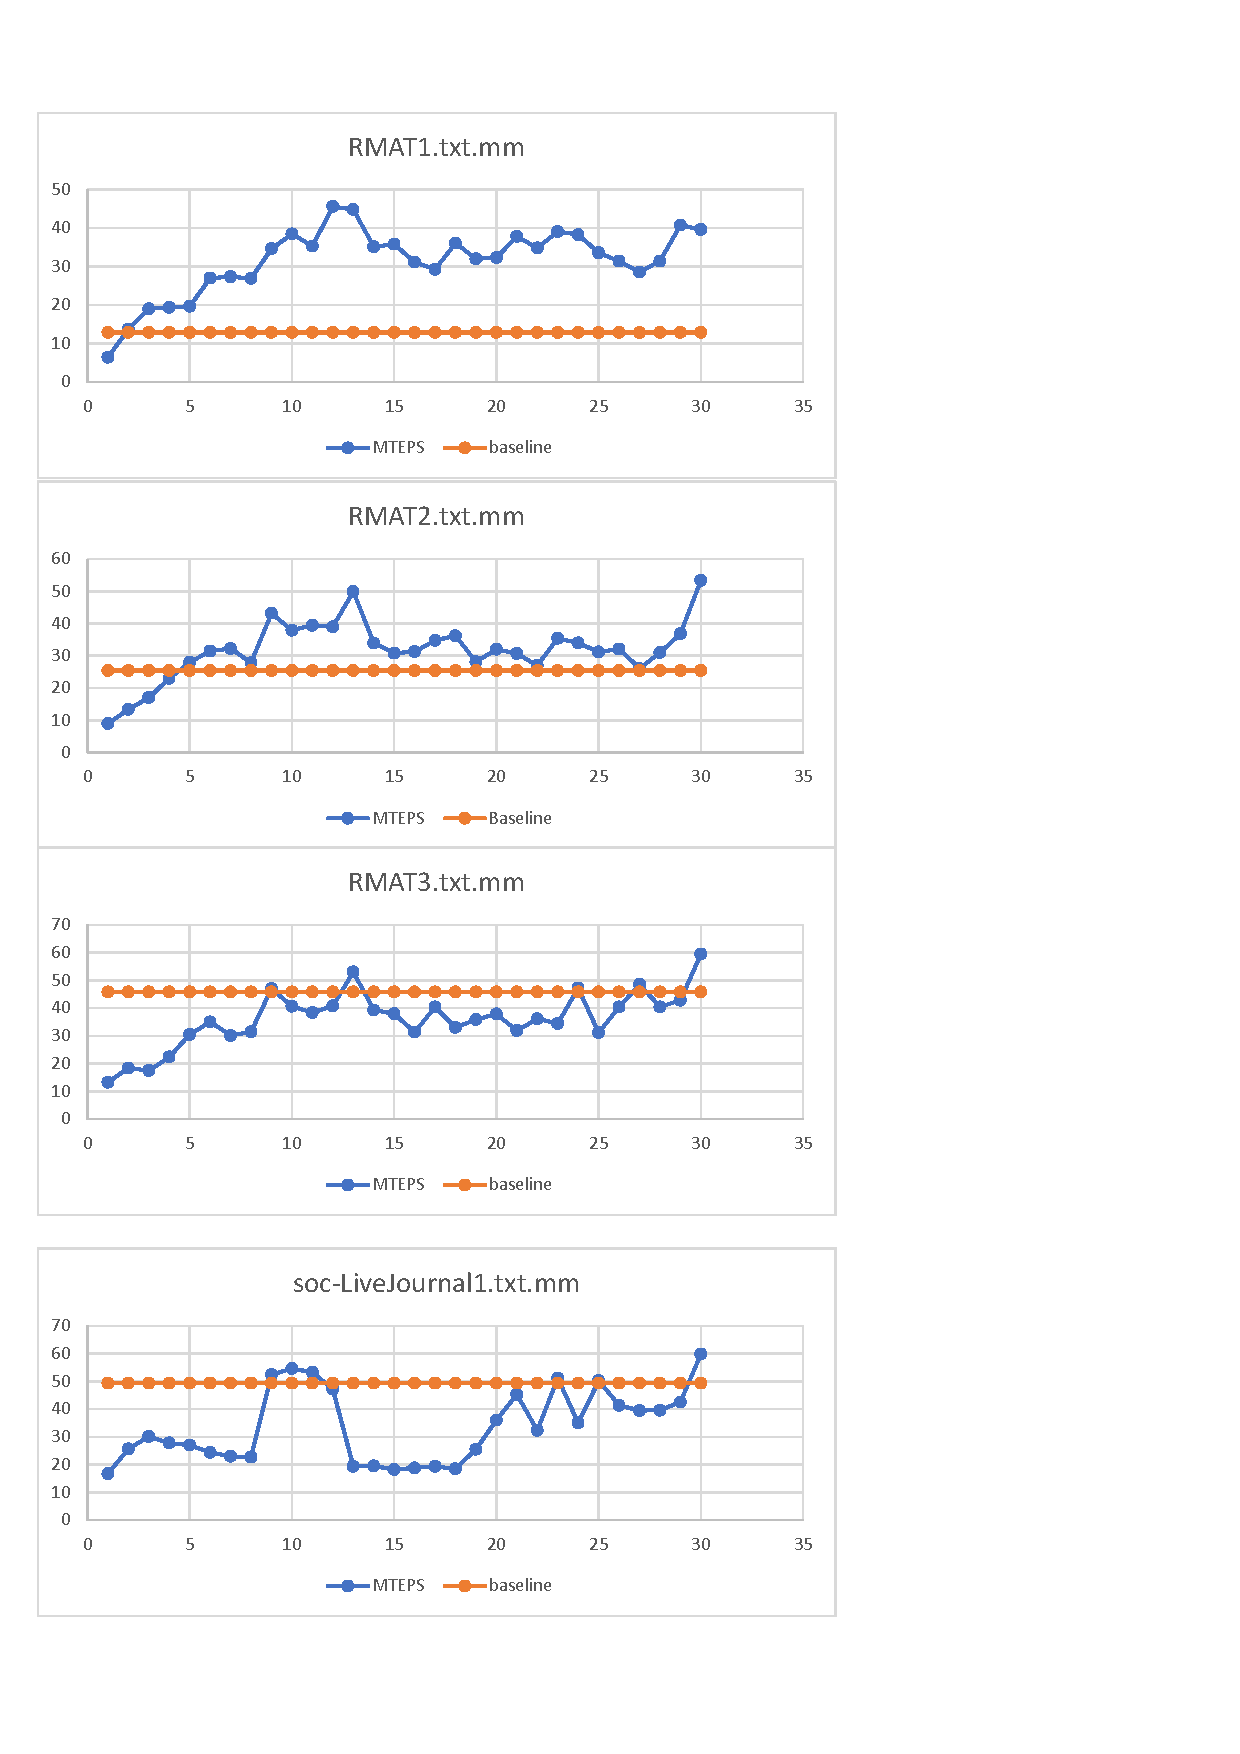
\includepdf[pages={1,2}]{performance.pdf}

\subsection{on local machine}

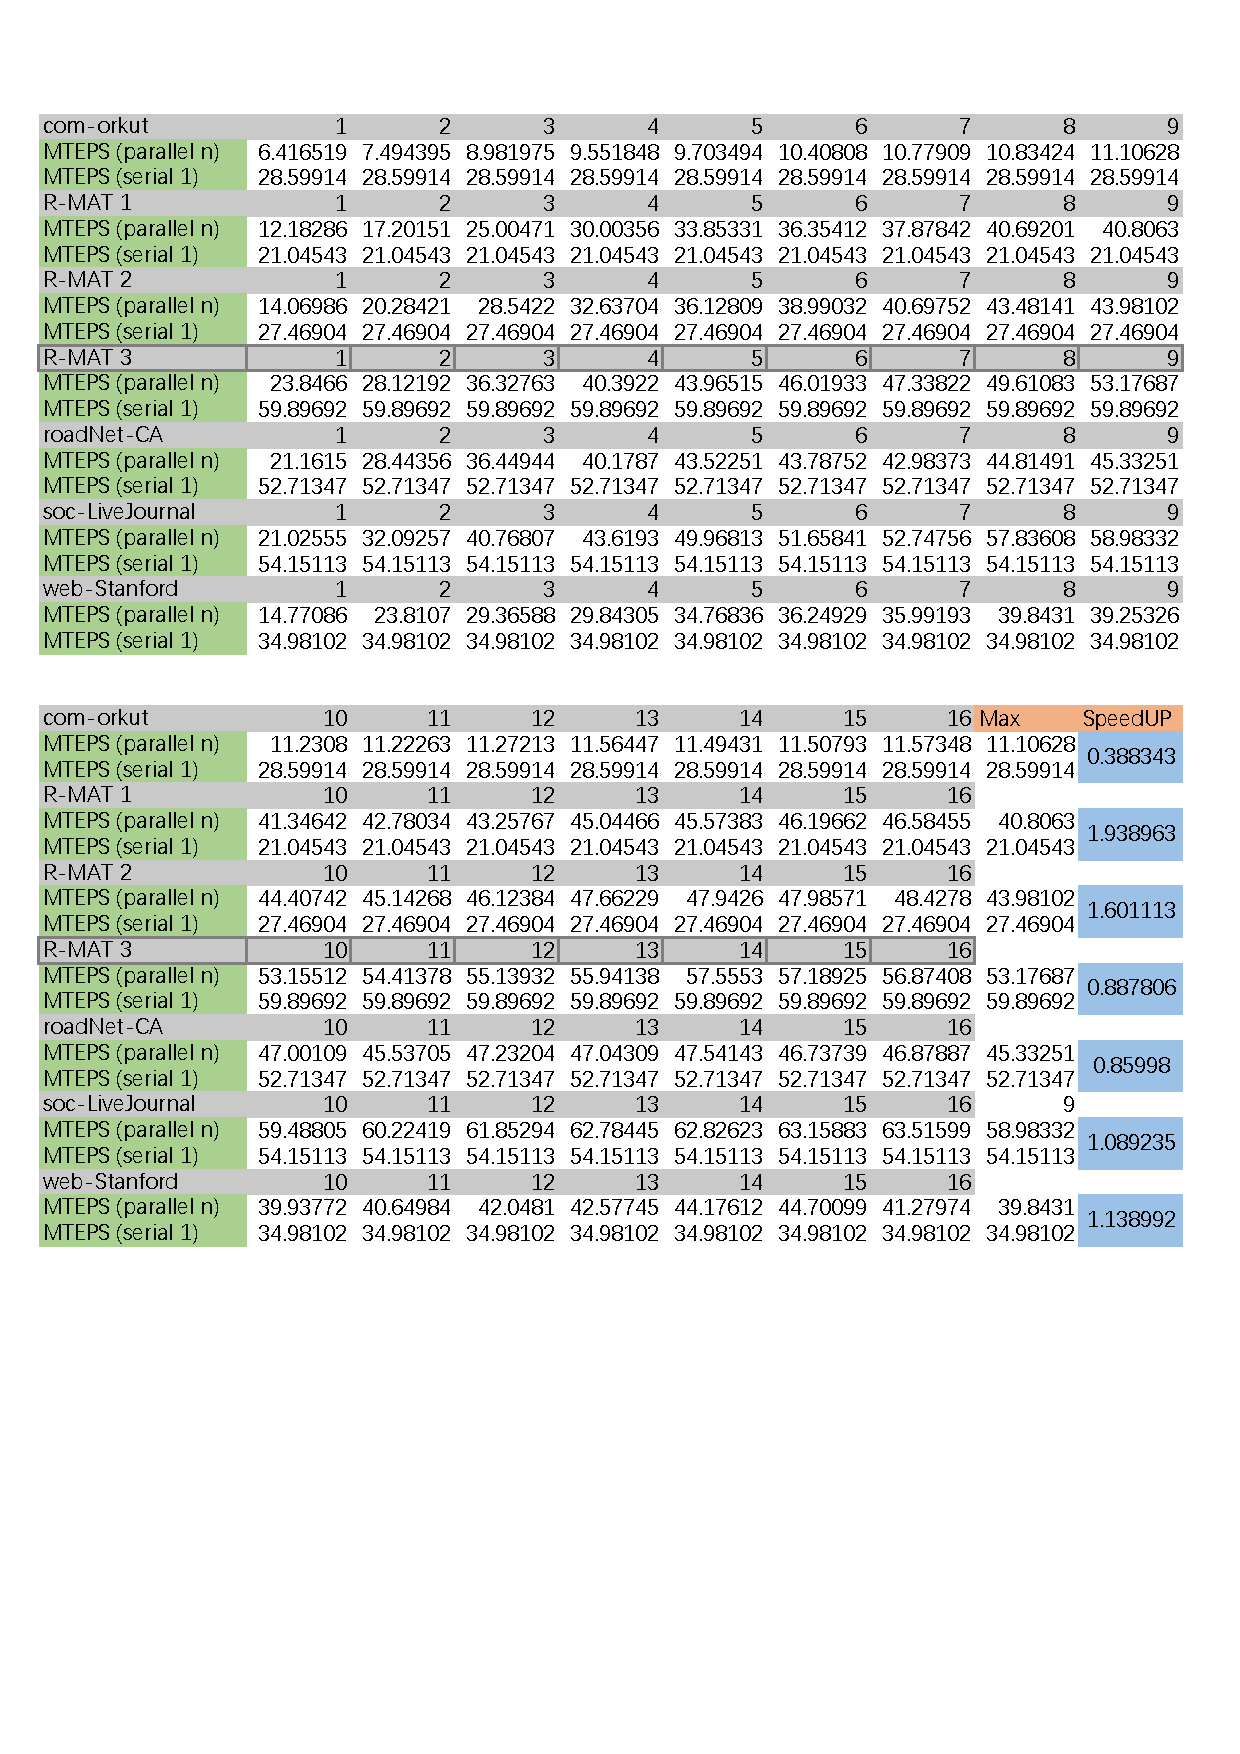
\includepdf[pages={1,2,3,4}]{performance-local.pdf}

\pagebreak


\printbibliography[
	heading=bibintoc,
	title={bibliography}
]

\end{document}
